\documentclass[a4paper,10pt]{article}
\usepackage[utf8]{inputenc}
\usepackage[]{algorithm2e}
\usepackage{pdfpages}
\usepackage{url}
\usepackage{biblatex}
\bibliography{./ref}
\usepackage{float}
%opening
\usepackage{listings}
\usepackage{titling} % Allows custom title configuration

\title{Distant Supervision for Numerical Relation Extraction} % Your article title


\begin{document}


\begin{titlepage}
    \centering
    \vspace*{\baselineskip}
    \rule{\textwidth}{1.6pt}\vspace*{-\baselineskip}\vspace*{2pt}
    \rule{\textwidth}{0.4pt}\\[\baselineskip]
    {\LARGE \color{blue} Distant Supervision for Numerical Relation Extraction}\\[0.2\baselineskip]
    \rule{ \textwidth}{0.4pt}\vspace*{-\baselineskip}\vspace{3.2pt}
    \rule{\textwidth}{1.6pt}\\[\baselineskip]
    \scshape
    Submitted in partial fulfillment of requirements for the degree of
    Master of Technology \par
    \vspace*{1\baselineskip}
     by \\[\baselineskip]
    {\large  Aman Madaan \vspace*{1\baselineskip} \\ Under the Guidance of Prof. Sunita Sarawagi,\\ Prof. Ganesh Ramakrishnan and Prof. Mausam\par}
       \begin{figure}[h]
 \centering
 \vspace*{13\baselineskip}
 
\includegraphics[bb=0 0 229 220,scale=0.35]{./iitb_logo.jpg}
 % iitb_logo.jpg: 229x220 pixel, 72dpi, 8.08x7.76 cm, bb=0 0 229 220
\end{figure}

    {\vspace*{1\baselineskip}  \itshape Department of Computer Science and Engineering \\ Indian Institute of Technology Bombay\par}
    \vfill
 
    {\scshape October, 2014} \\
    {\large }\par
  \end{titlepage}
\newpage
\maketitle

\tableofcontents
\newpage
\begin{abstract}
The task of numerical relation extraction poses new, hitherto untackled challenges. The bewildering amount of false positives, units, 
modifiers, time varying relations are just some of the issues that are non existent for standard relation extraction, but become 
crucial when numbers are involved.

We discuss molding distant supervision for numerical relation extraction. The standard one-to-one mapping using numbers as the second entity 
fails. Adding units help in improving the training data to a certain extent. The third heuristic, keyword based pruning further improves 
precision in the matches.
Analysis of the results from the three heuristics lead to a basic rule based extractor, which performs better than any of the heuristics.


\end{abstract}

\newpage
\section{Introduction}
Massive knowledge bases containing the entire information of the web in a neat, ready to process, structured form continue to be a part of an IR researcher's reverie.

This is not unexpected; such knowledge bases have potential of revolutionizing the way in which information is searched by users on the web or exchanged by machines among
themselves. 
Clearly, any progress towards a solution will have to deal with intricacies of how facts are expressed in the natural language.
It turns out that such intricacies are too many to exhaust. Years of research has went into the aforementioned goal, and still
there are plenty of loose screws. This report discusses one of them, numerical relation extraction.

We start with the problem definition, followed by an explanation of Distant supervision. We then present a summary of some of the
key works. Subsequently, we discuss casting standard distant supervision for numerical relation extraction and the improvements achieved using
Units and keywords. Finally, we discuss a simple rule-based relation extractor.


\subsection{Terminology}

\begin{itemize}

\item \textbf{a)Entity}
An entity is something that exists in itself, actually or hypothetically. \cite{wikientity}

\item \textbf{b)Relation}
A relation specifies a concept which binds two entities. For example, creator(Linux, Linus Torvalds).

\item \textbf{c)Mention}
 A piece of text which expresses a relation. For example, the sentence ``Linus Torvalds is the creator of Linux.''

\item \textbf{d)Match}
A mention expressing a relation $R$ is called a match for $R$. The criteria for deciding whether the mention $m$ is a match or not 
can vary. Presence of both the entities is, however, a mandatory condition.

\item \textbf{e)Extraction}
A 3-tuple $R(A, B)$ where $A$ and $B$ are entities related via a relation $R$.
\end{itemize}

\section{Problem}
Train extractors that can harness the Web for numerical relations, where relations are 3-tuples linking an entity
to a number. For example,
    \begin{itemize}
	\item  (India, \textbf{economy}, 1.842 trillion USD)
	\item  (China, \textbf{internet users},  590.56 million)
	\item  (USA, \textbf{land area}, 2,959,054 square mile)
    \end{itemize}

\section{Snowballing}
Let us motivate the idea by considering the following related problem:

Suppose we want to populate a repository of founders of companies, and all that we know
is that Elon Musk is the founder of SpaceX.
The problem can be divided into the following two parts, each of them rely on an intuition about how human 
beings form sentences in general.

\begin{itemize}
 
\item \emph{Given an entity pair, and a corpus of documents, find out all the sentences that
\textbf{express a relation} between the entity-pair.}

Command line ninjas will quickly think of the following solution:\\
grep -i 'entity1' sentences$\vert$ grep -i 'entity2'

The intuition behind this perhaps the most obvious solution is that \emph{a sentence
that houses both the entities can be expected to express a relation between them}.
A quick web search with the query ``entity1'' and ``entity2'' will show that this 
intuition is not out of the blue.

\item \emph{Find what makes these sentences special} \\
Sentence structure depends on the relation being expressed.
In verbose, if two sentences express the same relation, there will be (okay, there can be expected to be)
 \emph{features} that are similar in both of them. These include POS tags, words around the entities,
dependency path between the entities to name a few.

\end{itemize}
Putting together the intuitions above, we can solve the problem as follows:
Collect all the sentences which have SpaceX and Elon Musk in them, extract features 
from these sentences. Favor those features which repeat.
Now use this set of features to extract similar pairs from other sentences.
A fancier solution would be to reuse the extractions to learn more features, and continuing the process 
till the point of diminishing returns.

This seemingly shaky method actually works \cite{snowball} and is popular by the name of snowballing.

\section{Distant Supervision: Snowball scaled up}
\label{ds}
\subsection{Introduction}
If the idea of Snowball looks convincing, Distant supervision should follow naturally.
Earlier, we considered only one relation for one entity pair. Scale the amount of both of these up
and we have distant supervision.
The basic setup is as follows:
\begin{itemize}

\item \textbf{a) KB:} A knowledge base consisting of facts. The facts are 3-tuples; the entities and the corresponding relation.
For example:
\begin{center}

\begin{tabular}{|l|l|l|}
\hline
Entity & Entity & Relation \\
\hline
Donald Knuth & Wisconsin & Born In\\
Srinivasa Ramanujan & Erode & Born In \\
Alan Turing & London & Born In \\
Alon Musk & SpaceX & Founder Of\\
\hline
\end{tabular}
\end{center}

has 4 different facts

\item \textbf{b) Corpus}
The repository of text where we expect to find the sentences that express facts that we know.
We need another repository, called the test set, where we will run our extractor to obtain new facts.
These two can be the same.
\end{itemize}

\subsection{Distant Supervision Assumption}
Every sentence that has an entity pair ($e_1$, $e_2$) expresses the relation which exists between ($e_1$, $e_2$).
\subsection{Matching}
We next need to align our knowledge base with the corpus. This process is also called matching.

\begin{algorithm}[H]
 \KwData{Corpus C, Knowledge Base KB}
 \KwResult{Training data, D, A set of matches}
 Break C into a set of sentences, S\;
 \For{each sentence s in S}{
  let E = all entity pairs in s\;
  \For{each entity pair ($e_1$, $e_2$) in E}{
  \If{$\exists$ relation r in KB with r($e_1$, $e_2$)}{
    add s to D with label r
   } {
   
  }
  }
 }
 \caption{Distant Supervision: Matching}
\end{algorithm}


\subsection{Training}
Recall that obtaining the sentences which express a relation gives us training data, which 
we want to use to learn relation extractors, our goal.
There are several ways to achieve this, starting from the naive ways of training sentence 
level classifier extending to fancier graphical model based learning.
There are broadly two different ways of used in the literature for training extractors using the distant supervision data.
Earlier work on distant supervision used the training data to train classical classifiers, like naive bayes, LR and so on.
Recent work has shifted towards modeling extraction using graphical models.
\section{Survey}

The first distant supervision paper came out in 1999 \cite{craven}. The process has remained more or less the same since the first paper, with 
different works stemming out of either relaxations of different assumptions made by \cite{craven} or by using a smarter matching algorithm.

\subsection{Constructing Biological Knowledge Bases by Extracting Information from Text Sources, Craven and Kumlien 1999}
This was the first work to use distant supervision for creating a repository of biological facts. 
They targeted 5 different relations between Proteins, Tissues, Cell-Types, Diseases, Pharmacologic-Agents and Subcellular-structure.
A naive bayes based simple relation extractor is first described. The extractor works in 2 steps:  A classifier trained on hand labeled data
first labels whether a sentence \emph{can} express a particular relation. If yes, the sentence is searched for a pair of one of the 5 types
depending on the label and the fact is added to the database.
The authors note that it took an expert 35 hours to hand label the corpus. This forms the basis of motivating distant supervision based 
methods.The paper also identifies many areas of improvements, like a pair of entities taking up multiple relations, on which subsequent work has been
built up.

The authors obtain an improvement of around 9 precision points with distant supervision.
It is possible that the following points contributed to the improvement in scores:
\begin{itemize}
 \item Constrained entity set. Proteins and Tissues won't just appear together without any possible relation. 
 \item The corpus used was very well aligned with the knowledge base.
\end{itemize}

\subsection{Distant Supervision for the Web, Mintz et. al 2009}
This work revived the interest of the community around the problem of distant supervision.
The major contributions of this paper can be listed as follows:
\begin{itemize}
 \item \textbf{Distant Supervision for the Web}
 Craven and Kumlien had a limited knowledge base and a limited corpus to align it with.
 As the web exploded, the knowledge bases that became available were of the magnitude of FreeBase, and the
 corpus that can be aligned with it was the web. Mintz et. al bought this fact to the spotlight and sparked 
 a series of works.
 
 \item \textbf{Features}
 They designed a set of rich features that are used by researchers to date. These features include dependency paths, POS tag sequences, word sequences to name a few.
 
\end{itemize}

\subsection{Learning 5000 relation extractors} \cite{rel}
The number of relations typically used in the works were limited to the range of 30-40. 
This work targeted 5000 relations, which is a big jump. To fight sparsity that will arise 
in the training data due to a large number of classes, they also train a top level classifier
which decides which extractor should be used for a particular document. Not all the extractors 
are employed for a given document.

\subsection{Riedel et. al}\cite{riedel}
Distant supervision assumption does not really holds when the knowledge base is not well aligned with the corpus.
Another way of saying this would be that the corpus can be expected to consist of sentences that can host entity pairs
in a wide range of contexts, and the sentences may have nothing to do with the relations in which the entity pairs appear.
They take the example of the relation ``nationality''. A wide range of popular entities that are born in the country 
will be mentioned in the sentences that may have nothing to do with the fact that they were born in that country.
In such cases, it can be argued that the training data generated will be extremely noisy and will lead to poor extraction 
performance. Riedel et. al relax the distant supervision assumption.

\subsection{MultiR}\cite{multir}
Some of the entity pairs can occur in multiple relationships. For example, an athlete usually \emph{plays for} the 
country they are \emph{born in}. The \emph{CEO of} a company also \emph{works for} it. The techniques discussed till now are 
focused on extracting only one of the relations for an entity pair. MultiR relaxes one relation per entity-pair assumption. 
(Hence the name, multi-relation). MultiR achieves this by modeling both sentence level and corpus level extraction decision.
The graphical model is as shown in figure \cite{fig:multir}] (taken from [\ref{multir})
\begin{figure}[H]
 \centering
 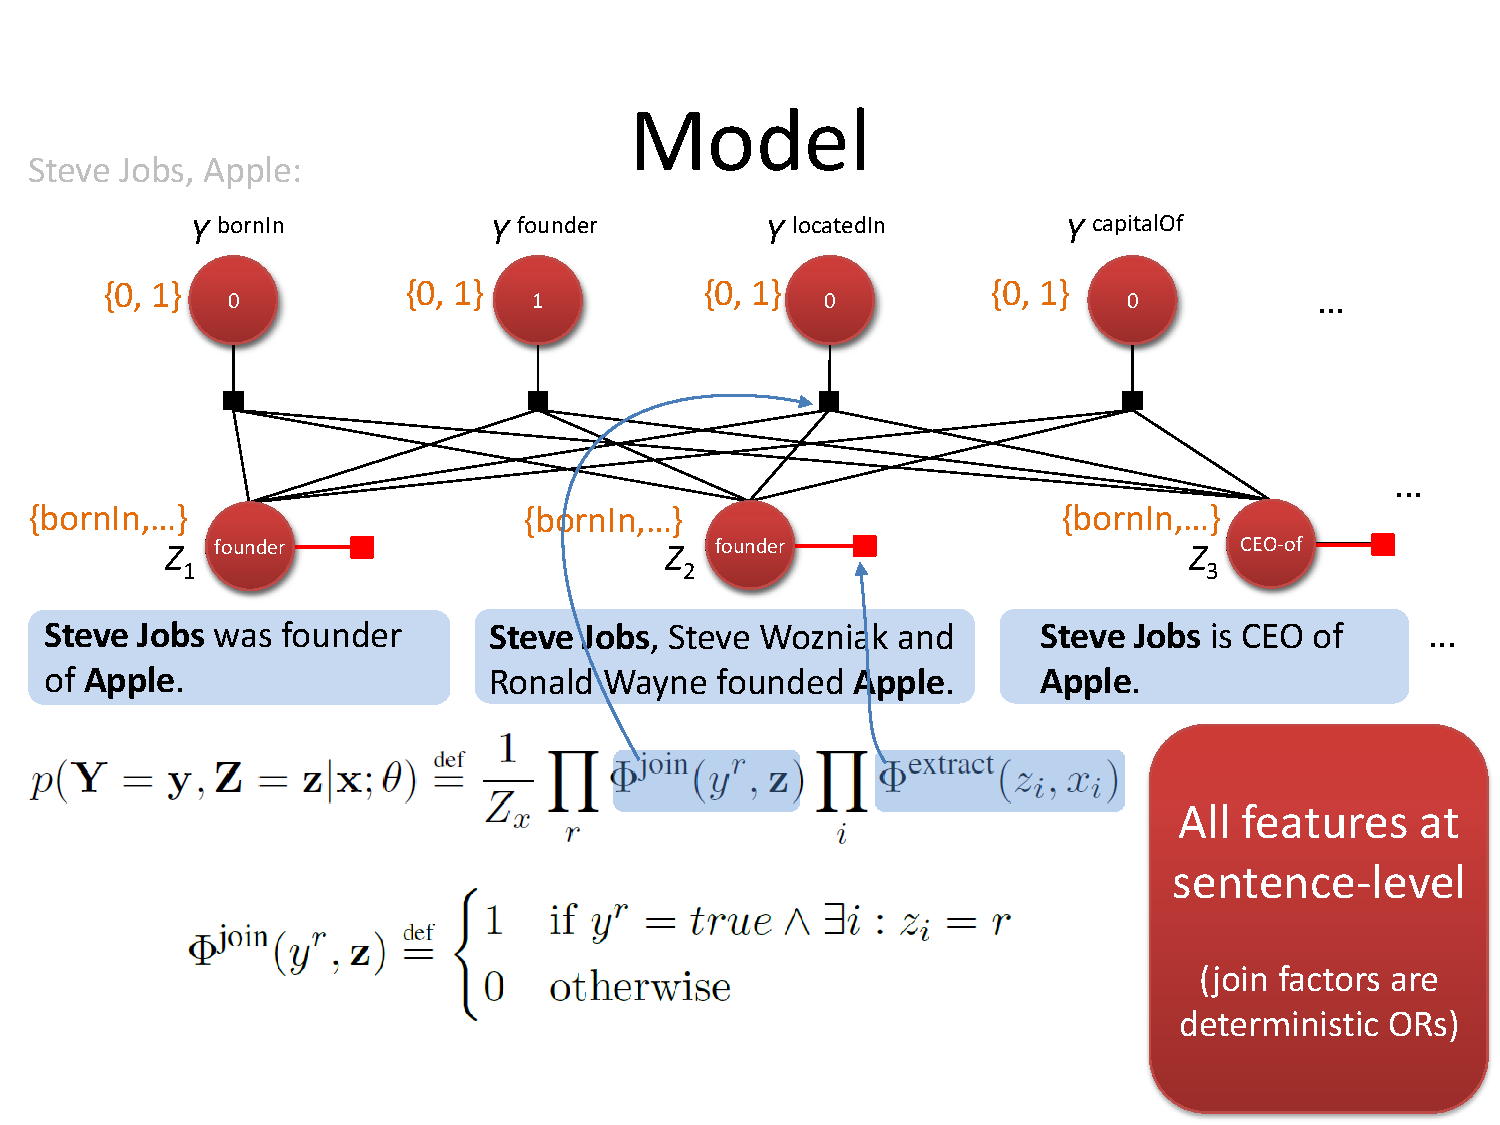
\includegraphics[bb=0 0 720 540,scale=0.45]{./multirmode1.pdf}
 % multirmode1.pdf: 720x540 pixel, 72dpi, 25.40x19.05 cm, bb=0 0 720 540
 \caption{MultiR Graphical Model}
 \label{fig:multir}
\end{figure}

There are two different types of nodes in the model:
\begin{itemize}

\item \textbf {a) Sentence Level extractions, Z:}
The cardinality of these variables is equal to the number of targeted relations + 1 for ``no attachment'', which means that 
the sentence expresses no relation. This is important for relaxation of the DS assumption.

\item \textbf{b) Corpus level extraction, Y:}
The Ys are the binary variables, one for each relation. $Y_i$ takes the value of 0 or 1 depending on whether the $ith$ relation is expressed 
in the corpus or not.
\end{itemize}

There are 2 factors:
\begin{itemize}
\item \textbf{a) Factors local to Z} These factors capture the likelihood of a sentence belonging to one of the relations.
The usual technique of representing factor tables in log-linear forms is used. The features are as defined by 
\cite{mintz}.

\item \textbf{b) Factors between Y and Z} These factors ensure that the probability mass is divided only amongst the possible extractions.
As shown in the figure, the factor takes a value of 1 only if the corpus level bit is 1 i.e. that relation exists at corpus level \textbf{and} 
at least one of the sentences also expresses it.
\end{itemize}
  
  
\section{Numerical Relations}
Numerical relations are much like the usual entity-entity relations, just more problematic.
What we call a \emph{numerical relation} will usually be called an attribute colloquially. 
For example, Camel and 215cm are related via the relation ``Average Height''.

\section{Numerical Relation extraction using MultiR}
The problem of numerical relation extraction can be easily cast into the distant supervision framework.
Recall from section \cite{ds} that we need a corpus and a knowledge base to generate the training data for distant supervision.
We also need to fix on the set of relations that will be targeted. 

\subsection{Relations}
The following 10 relations were chosen for our experiments:
 \begin{center}
 \begin{table}[H]
\begin{tabular}{|l|l|}
\hline
Relation Name & Relation Code \\
\hline
Land area (sq. km)&AG.LND.TOTL.K2\\
Foreign direct investment, net (current US\$)&BN.KLT.DINV.CD\\
Goods exports (current US\$)&BX.GSR.MRCH.CD\\
Electricity production (kWh)&EG.ELC.PROD.KH\\
CO2 emissions (kt)&EN.ATM.CO2E.KT\\
Pump price for diesel fuel (US\$ per liter)&EP.PMP.DESL.CD\\
Inflation, consumer prices (annual \%)&FP.CPI.TOTL.ZG\\
Internet users (per 100 people)&IT.NET.USER.P2\\
GDP (current US\$)&NY.GDP.MKTP.CD\\
Life expectancy at birth, total (years)&SP.DYN.LE00.IN\\
Population (Total)&SP.POP.TOTL\\
\hline
\end{tabular}
\caption{Selected Relations}
\label{rels}
\end{table}
\end{center}

The relations were selected keeping in mind the availability of sentences which potentially express these facts
and to have some diversity in units.

\subsection{Knowledge base}
Our knowledge base was derived from \url{data.worldbank.org}.
It has 4371979 numerical facts about 249 countries ranging over 1281 different attributes. 
Table \cite{fig:kb} shows a sample.

\begin{table}[H]
\centering
\begin{tabular}{|l|l|l|}
\hline
Country id & Number & Relation \\
\hline
/m/04g5k&3126000130&EG.ELC.PROD.KH\\
/m/02k8k&1969.179&EN.ATM.CO2E.KT\\
/m/06nnj&332315&SP.POP.TOTL\\
/m/019rg5&55.020073&SP.DYN.LE00.IN\\
/m/05sb1&19974.148&EN.ATM.CO2E.KT\\
/m/05v8c&10000000000&EG.ELC.PROD.KH\\
/m/03spz&7639000100&EG.ELC.PROD.KH\\
/m/06vbd&44249.688&EN.ATM.CO2E.KT\\
/m/0d060g&51.3&IT.NET.USER.P2\\
/m/05qkp&62.298927&SP.DYN.LE00.IN\\
\hline
\end{tabular}
\caption{A Sample of our KB}
\label{fig:kb}
\end{table}


\section{L'homme propose, et Dieu dispose}
Our life would have been simpler if MultiR would do the desired; extract the numerical relations from the corpus provided
information about some of the numerical relations. However, as table \cite{vanillatable} shows, the quality of training data
is so poor that not much can be expected from the extractor obtained.

\begin{center}
\begin{table}[H]

\resizebox{\linewidth}{!}{% Resize table to fit within \linewidth horizontally

\begin{tabular}{|l|l|l|l|l|}
\hline
Relation&Total Matches&Sampled Matches&True Matches&Precision(\%)\\
\hline
Land Area&1884&15&\textbf{1}&\textbf{6.7}\\
Foreign Direct Investment&0&0&0&0\\
Goods Export&0&0&0&0\\
Electricity Production&381&10&0&0\\
$CO_{2}$ Emission&0&0&0&0\\
Diesel Prices&8491&15&0&0\\
Inflation(\%)&8689&15&0&0\\
Internet Users(\%)&182319&40&0&0\\
GDP(\$)&0&0&0&0\\
Life Expectancy&267&10&0&0\\
Total Population&0&0&0&0\\
\hline
\end{tabular}}
\caption{Vanilla Match}
\label{vanillatable}
\end{table}
\end{center}

The model not doing well may mean several things. Low quality training data being one of the primary reasons.
Indeed, it turned out that vanilla distant supervision leads to an \textbf{unprecedented} amount of false positives, which are the root cause
of everything that went wrong in the distant supervision pipeline.

\subsection{Numbers and False positives}
Why would numbers lead to false positives in the first place?
The problem stems from the fact that numbers have no identity of their own; they represent count of
some real entity or phenomenon.

\begin{itemize}
 \item \textbf{Numbers can appear in many more contexts with an entity}
The number of ways in which any two entities can appear together
in a sentence is far less than the number of ways in which a number and a quantity can appear
together. For example, Consider the entity pair “Bill Gates” and “Microsoft” and the entity-number
pair “Bill Gates” and “3” (say). While former will usually co-occur in finite contexts (Founder,
CEO, Evangelist etc.), the latter may co-occur anywhere Bill Gates happen to be around something
which is 3, the number of cars, billion dollars donated, number of units headed, position in the
company, number of business units shutdown by Microsoft and so on.
\item The situation is worse for smaller whole numbers, which are more frequent. This intuitively makes
sense as we are more often see 2,3 or 11 than 111212233 or 11.42143.
\item \textbf{The match mines}

During the initial phases of our experiments, we stumbled upon the \emph{match mines}
These were basically huge tables, world cup scores of all the matches played and so on.
A couple of such sentences were responsible for 21\% of the matches!
It is easy (and very important) to get rid of such sentences. For subsequent runs, we first sort the sentences by length and then remove
top 1000 of them.
\end{itemize}


\section{Fighting False Positives with units}
Analyzing results of plain matching made it clear that units will help in improving both precision
(by eliminating matches where the unit is not present) and recall (increasing matches by
canonicalization of numbers and conversion to SI units). We found that though units helped in
drastically cutting down the number of false positives (match mines were completely eliminated),
and helped recall (lots of good matches for Land area and Population), the number of false positives
was still a trouble. The number of false positives was typically high for cases where the unit was
percentage, since it is again a very generic unit. For other relations too, the number of false
positives was very large. The large number of false positives, apart from degrading quality of the
model, make evaluating the quality of matcher very difficult.

As the next step, we integrated Prof. Sunita's unit extractor in the distant supervision pipeline.
Concretely, we fed the corpus to the unit extractor to get information of the following form
(sample):
\begin{center}
 
\begin{tabular}{|l|l|}
\hline
Sentence ID & Numbers with units \\
\hline
2000064&172010.0::64:72;500.0::157:160;\\
2000077&75.0:united states dollar:17:19;2010.0::55:67;29.0::69:70;\\
2000080&50.0::47:49;\\
2000112&172009.0::56:64;\\
2000113&0.10000000149011612::58:61;\\
2000120&3.15564E7:second:113:115;1.0::131:132;\\
\hline
\end{tabular}

\end{center}

Where the format of a single match is:

\emph{sentence id [TAB] Number, unit, startOffset, endOffset;Number2,unit,startOff,endOff}
The knowledge base was also converted to SI units.
We see lots of true positives for attributes that take value in the higher range. The number of false
positives has also drastically decreased. Units have been particularly helpful in dealing with the so
called “match mines”, sentences which have lots of country names and numbers, like score tallies.

\subsection{Results}
As table \cite{fig:resunits} shows, units help, but not as much as we would have expected.
\begin{center}
\begin{table}[H]
 \resizebox{\linewidth}{!}{% Resize table to fit within \linewidth horizontally
\begin{tabular}{|l|l|l|l|l|}
\hline
Relation&Total Matches&Sampled Matches&True Matches&Precision(\%)\\
\hline
\textbf{Land Area} &98	& 40 & 32 &80\\
Foreign Direct Investment & 791 & 40& 1&2.5\\
Goods Export&816&40&3&7.5\\
Electricity Production&19&19&0&0\\
$CO_{2}$ Emission&196&40&2&5\\
Diesel Prices&2&2&2&100\\
Inflation(\%)&27598&40&0&0\\
Internet Users(\%)&24639&40&0&0\\
GDP(\$)&1790&40&0&0\\
Life Expectancy&3081&40&0&0\\
\textbf{Total Population}&5225&40&11&27.5\\
\hline

\end{tabular}}
\caption{Unit Based}
\label{fig:resunits}
\end{table}
\end{center}

There can be several reasons for this.
 \begin{itemize}
  \item Attributes with Unit \% (inflation, internet user \%), are affected by stock data that is heavily present in the news corpus.
  \item Relations FDI, Goods Export, GDP have almost similar values, thus, an (entity, number) pair matches all of the three relations. 
  \end{itemize}
  
The analysis indicates that we might need some relation specific heuristics.
 

\section{Numbers are weak entities: a case for keywords}

\subsection{Motivation}
Matches from unit extraction showed that in some cases, the sentence that supposedly labeled as a
match for a particular relation has no mention of the relation itself at all.
For example, consider:
“In eurozone powerhouse Germany, industrial orders jumped 3.2 percent in June, official data
showed Thursday, with foreign demand behind a sharp rebound following a surprise drop in May.”
In this sentence, (Germany, 3.2) was considered as a match pair for the relation Internet user
percent. Clearly, it has nothing to do with it.

\subsection{Numerical Relations are Explicit}
A key observation that can be made by going through the sentences that express numerical relations
is that one cannot be too poetic while forming a sentence that is supposed to state a numerical fact.
This is in stark contrast with sentences expressing relations between entity pairs, wherein the
underlying relation might be implicit. If we want to state GDP of a country in a sentence, there is no
escape from the words like “GPD” or “gross domestic product” and the likes * .

Compare this with a sentence that must relate Microsoft and Bill Gates. A few ways of stating that
Microsoft was founded by Bill Gates can be enumerated as follows:
\begin{itemize}
\item Bill Gates is the founder of Microsoft
\item Bill Gates founded Microsoft
\item Bill Gates is the father of Microsoft
\item Bill Gates laid the foundation stone of Microsoft
\item Bill Gates started Microsoft
\end{itemize}

If this is indeed true, imposing an additional constraint of keyword being present in a sentence in
addition to the fact being present can help in cutting down the number of false positives. We note
that such a pruning is possible only in case of numerical relations. As mentioned earlier, for real
world entity pairs, co-incidental matches will be rarer and a constraint on the relation word being
present will be too restrictive.
\subsection{Approach}
Let $M_r$ be the set of matches obtained by standard unit + distance based matching for a relation r.
We prune $M_r$ by picking only sentences which contain one of the words in the set keywords(r).
The sets keywords(r) are manually crafted and are listed in table \cite{fig:kw}.

\begin{center}
\begin{table}
 \begin{tabular}{|l|l|}
\hline \\
 Relation Keywords & (case insensitive)\\
\hline
 Internet User \% &"Internet"\\
Land Area &"area", "land", "land area"\\
Population &"Population"\\
Diesel &"diesel"\\
GDP &"Gross domestic", "GDP"\\
CO2 &"Carbon", "Carbon Emission", "CO2"\\
Inflation &"Inflation", "Price Rise"\\
FDI &"Foreign", "FDI"\\
Goods Export & "goods"\\
Life Expectancy & "life", "life expectancy"\\
Electricity Production & "Electricity\\
\hline
\end{tabular}
\caption{Keywords for Relations}
\label{fig:kw}
\end{table}
 \end{center}

\subsection{Results}
The results indicate that keywords help a lot. 
\begin{table}[H]
\resizebox{\linewidth}{!}{% Resize table to fit within \linewidth horizontally 
\begin{tabular}{|l|l|l|l|l|}
\hline
Relation&Total Matches&Sampled Matches&True Matches&Precision(\%)\\
\hline
\textbf{Land Area}&61&40&\textbf{30}&\textbf{75}\\
Foreign Direct Investment&8&0&0&0\\
Goods Export&4&4&0&0\\
Electricity Production&0&0&0&0\\
$CO_{2}$ Emission&16&16&2&12.5\\
Diesel Prices&2&2&2&100\\
\textbf{Inflation(\%)}&3853&40&25&62.5\\
Internet Users(\%)&308&40&7&17.5\\
GDP(\$)&0&0&0&0\\
\textbf{Life Expectancy}&99&40&15&37.5\\
\textbf{Total Population}&607&40&24&60\\
\hline

\end{tabular}
}
\caption{Keyword Based}
\label{fig:kwres}
\end{table}



\section{A summary of the three heuristics}

Before discussing the results, let us summarize the heuristics:
\begin{itemize}
\item \textbf{a) Vanilla:} A sentence having a country-number pair $c-n$ is called a match for a relation $R$ if $R(c,n)$ is a fact in the KB.
\item \textbf{b) Unit Based:} Feed the corpus to a unit extractor, extract normalized numbers along with units. During matching, both the normalized value of a number
and the unit are considered.
\item \textbf{c) Keyword based:} In addition to matching number and unit, also check whether one of the keywords for a relation is present. 
\end{itemize}

\begin{figure}[H]
 \centering
 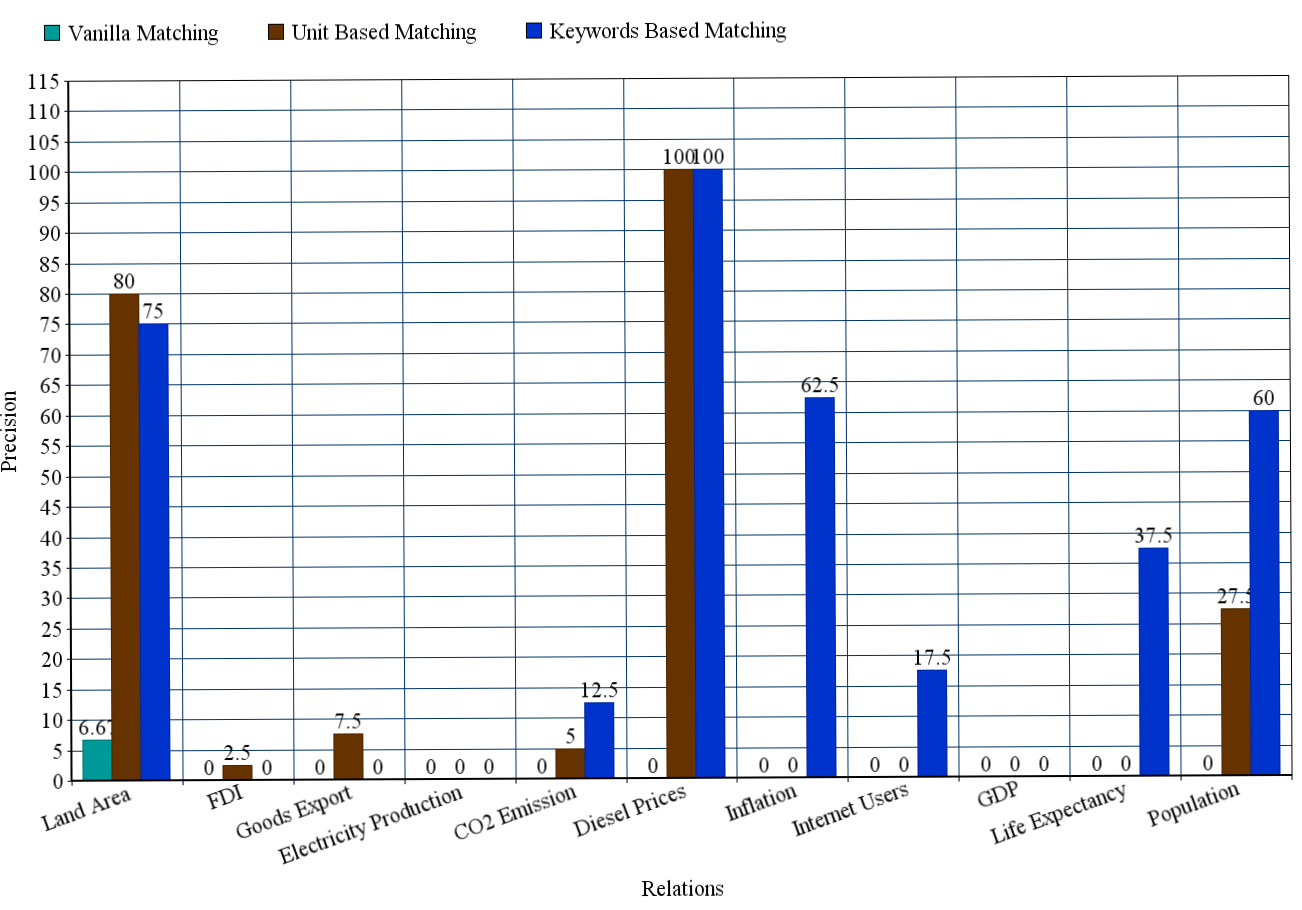
\includegraphics[bb=0 0 1360 1000,scale=0.25]{./results.png}
 % results.png: 1360x1000 pixel, 72dpi, 47.98x35.28 cm, bb=0 0 1360 1000
 \caption{A comparison of the three heuristics}
 \label{fig:comp}
\end{figure}



\section{Rule Based Extraction}

\subsection{Peculiarity of Numerical Relations}
Analyzing a number of sentences expressing numerical relations lead to several insights as already discussed.
\begin{itemize}
 \item \textbf{Keywords} Sentences expressing numerical relations can be expected to be explicit about the relation being expressed.
 Stated another way, we can expect presence of certain keywords that might help in identifying relations.
 \item \textbf{Modifiers} A large number of false positives stem out of mentions where a change in the numerical attribute is mentioned.
\end{itemize}

\subsection{Dependencies}
Dependencies are grammatical relation between two words, governor and dependent.
The relation captures the way in which one of the words is affected by the other.
For example, consider the sentence:
``The red ball was lost''
The dependencies are:
\begin{itemize}

\item \textbf{amod(ball,3,red,2)} ``Red'' is an adjective for ``ball''
\item \textbf{det(ball,3,The,1)}  ``the'' is a determiner of ``ball''
\item \textbf{nsubjpass(lost,5,ball,3)}	``ball is the subject of lost''
\item \textbf{auxpass(lost,5,was,4)}	``was is an auxiliary of lost''
\end {itemize}

\subsection{Dependency Path}
We define a dependency path between two words ``A'' and ``B'' as the shortest path between them in the dependency graph.
The dependency graph consists of one node for each of the words, and the dependencies are the collapsed typed dependencies 
as obtained from the stanford dependency parser. \cite{corenlp}. 
Figure \cite{fig:1} shows dependency graph for ``The estimated 2014 population of Zambia is 15,200,000, which ranks 70th in the world.''
\begin{figure*}
 \centering
 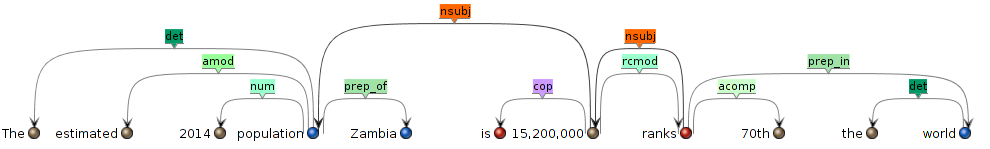
\includegraphics[bb=0 0 990 149, scale = 0.4]{./dep.png}
 % dep.png: 990x149 pixel, 72dpi, 34.92x5.26 cm, bb=0 0 990 149
 \caption{Dependency Graph}
 \label{fig:1}
\end{figure*}


\subsection{Relation extraction using dependency paths}
Intuitively, it makes sense that the entities which are related will have some dependence on each other in the sentence 
expressing the relation. If this is true, we can expect the following simple rule to work.
Let $P$ be the set of words in the path between a Country $C$ and a number $N$. Then, for $C$-$N$ to be an extraction for a relation
$R$, the following should hold:
  \begin{itemize}
   \item $P$ \textbf{should have} a word $w$ such that $w$ $\in$ $keywords(R)$
   \item \textbf{should not have} any word $w$ such that $w$ $\in$ $modifiers$
  \end{itemize}
  
Here $modifiers$ is a set of modifying words. The set is formed of the words like {``Increased, Decreased, 
Changed''}.

\subsection{Example}
Consider the sentence:
``The estimated population for 2014 of the Australian continent	is about 36.25 million people''
and the Country-Number pair (Australian, 36.25)
The dependency graph of the sentence is as shown in figure \cite{pos}.
\begin{figure}[H]
 \centering
 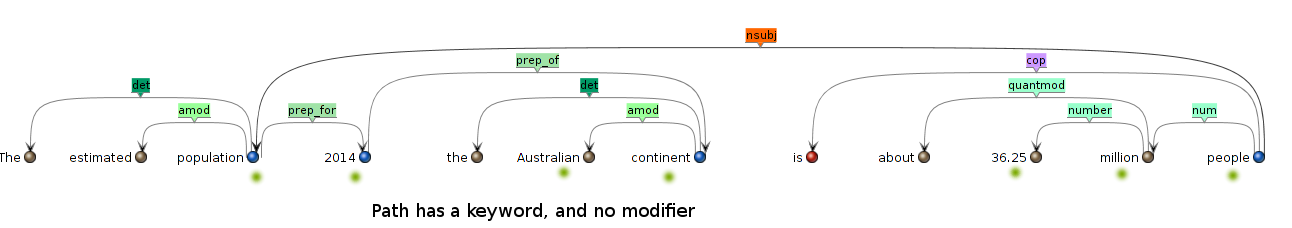
\includegraphics[bb=0 0 1292 228,scale=0.3]{./dep_pos.png}
 \label{pos}
 % dep_pos.png: 1292x228 pixel, 72dpi, 45.57x8.04 cm, bb=0 0 1292 228
\end{figure}
The path between Australia and 36.25 has ``people'', so this will be an extraction.

If we modify the sentence to:
``The estimated population for 2014 of the Australian continent	increased by about 3.25 million people''

The path will additionally have a modifier, ``increased'', and thus there won't be any extraction.
\begin{figure}[H]
 \centering
 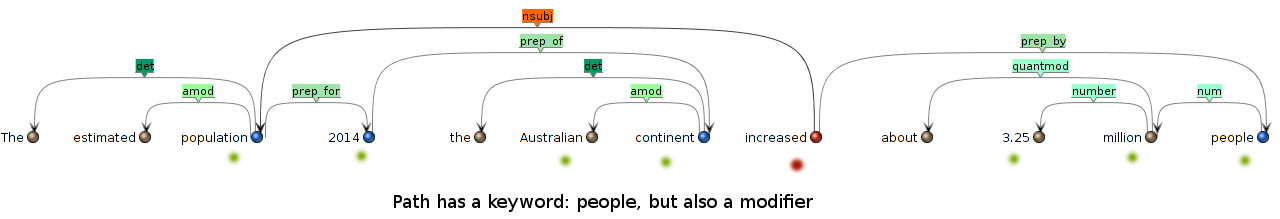
\includegraphics[bb=0 0 1292 228,scale=0.3]{./dep_neg.png}
 % dep_pos.png: 1292x228 pixel, 72dpi, 45.57x8.04 cm, bb=0 0 1292 228
 \label{neg}
\end{figure}




\subsection{Results}
\subsubsection{Precision and Recall}
The extractor was applied to 30 sentences expressing 23 different relations.
\begin{tabular}{|l|l|l|}
\hline
& Relations Present & Relations not Present (False positives) \\
\hline
Extracted & 16 & 17 \\
\hline
Not Extracted & 7 & N/A \\
\hline
\end{tabular}
 \begin{itemize}
  \item Precision: 48.4\%
  \item Recall: 69.6\%
 \end{itemize}

The precision should increase further on applying unit based pruning.

\subsubsection{Example Extractions}
\begin{tabular}{|l|} 
\hline
Sentence $\rightarrow$ Extraction \\
\hline
At 3.71 million square miles (9.62 million km2) and with around 318 million people,\\ 
the US is the world's 3rd or 4th-largest country by total area and third-largest by population. \\$\rightarrow$ POP( US, 318) \\
\hline
The land area \cite{hoffmann2011knowledge} of the contiguous US is 2,959,064 square miles (7,663,941 km2)\\ $\rightarrow$  AGL( US, 2,959,064), AGL( US, 7,663,941) \\
\hline
With 1,210,193,422 residents reported in the 2011 provisional census,\\ 
India is the world's second-most populous country.\\\ $\rightarrow$ POP( India, 1,028,737,436)\\ 
\hline
According to an official estimate for 1 June 2014, the population of Russia is 143,800,000.\\ $\rightarrow$
POP( Russia, 1), POP( Russia, 2014), POP( Russia, 143,800,000) \\
\hline
\end{tabular}

\section{Conclusion}
Though numerical relation extraction has been Numerical relation extraction 
%\begin{thebibliography}{9}

\bibitem{A} \label{thepaper} Kulkarni, Sayali, et al. ``Collective annotation of Wikipedia entities in web text.'' Proceedings of the 15th ACM SIGKDD international conference on Knowledge discovery and data mining. ACM, 2009.

\bibitem{B}  \label{thesite} \url{http://www.cse.iitb.ac.in/~soumen/OWI/Slides/}

\bibitem{C} \label{thesurvey} William Cohen's Survey available at \ref{thesite}

\bibitem{The Wikipedia Page} \label{thewiki} \url{http://en.wikipedia.org/wiki/Named-entity_recognition}
\bibitem{D} \label{stanfordner} \url{http://nlp.stanford.edu/software/CRF-NER.shtml}

\bibitem{E} 

\label{mw}
Milne, David, and Ian H. Witten. ``Learning to link with wikipedia.'' Proceedings of the 17th ACM conference on Information and knowledge management. ACM, 2008.

\bibitem{F}{ws} \label{ws} \url{http://www.worldwidewebsize.com/}

\bibitem{G} \label{wikistats} \url{http://en.wikipedia.org/wiki/Wikipedia:Statistics}

\bibitem{F} \label{wikify}
Mihalcea, Rada, and Andras Csomai. ``Wikify!: linking documents to encyclopedic knowledge.'' Proceedings of the sixteenth ACM conference on Conference on information and knowledge management. ACM, 2007.

\bibitem{H} \label{aida}
Hoffart, Johannes, et al. ``Robust disambiguation of named entities in text.'' Proceedings of the Conference on Empirical Methods in Natural Language Processing. Association for Computational Linguistics, 2011.

\bibitem{I} \label{kpsim}
Hoffart, Johannes, et al. "Kore: keyphrase overlap relatedness for entity disambiguation." Proceedings of the 21st ACM international conference on Information and knowledge management. ACM, 2012.

\bibitem{J} \label{relgram}
Balasubramanian, Niranjan, Stephen Soderland, and Oren Etzioni. "Rel-grams: a probabilistic model of relations in text." Proceedings of the Joint Workshop on Automatic Knowledge Base Construction and Web-scale Knowledge Extraction. Association for Computational Linguistics, 2012.

\bibitem{H} \label{cohschemas}
Balasubramanian, Niranjan, Stephen Soderland, and Oren Etzioni Mausam. "Generating Coherent Event Schemas at Scale." Proceedings of the Empirical Methods in Natural Language Processing. ACM (2013).

\bibitem{I} \label{lesk}
Michael Lesk. 1986. Automatic sense disambiguation using machine readable dictionaries: how to tell a pine cone from an ice cream cone. In Proceedings of the 5th annual international conference on Systems documentation (SIGDOC '86), Virginia DeBuys (Ed.). ACM, New York, NY, USA, 24-26. DOI=10.1145/318723.318728 http://doi.acm.org/10.1145/318723.318728

\bibitem{J} \label{wordnet}
http://wordnet.princeton.edu/wordnet/

\bibitem{K} \label{yago}
Suchanek, Fabian M., Gjergji Kasneci, and Gerhard Weikum. "Yago: a core of semantic knowledge." Proceedings of the 16th international conference on World Wide Web. ACM, 2007.

\bibitem{L} \label{dbpedia}
Auer, Sören, et al. "Dbpedia: A nucleus for a web of open data." The semantic web. Springer Berlin Heidelberg, 2007. 722-735.

\bibitem{M} \label{patty}
Nakashole, Ndapandula, Gerhard Weikum, and Fabian Suchanek. "PATTY: a taxonomy of relational patterns with semantic types." Proceedings of the 2012 Joint Conference on Empirical Methods in Natural Language Processing and Computational Natural Language Learning. Association for Computational Linguistics, 2012.

\bibitem{N} \label{freebase}
Bollacker, Kurt, et al. "Freebase: a collaboratively created graph database for structuring human knowledge." Proceedings of the 2008 ACM SIGMOD international conference on Management of data. ACM, 2008.

\bibitem{O} \label{mmd}
Iyer, Arun, Saketha Nath, and Sunita Sarawagi. "Maximum Mean Discrepancy for Class Ratio Estimation: Convergence Bounds and Kernel Selection." Proceedings of The 31st International Conference on Machine Learning. 2014.

\bibitem{Q} \label{aidafeature}
Using Structured learning for named entity disambiguation, \url{www.cse.iitb.ac.in/~amanmadaan/structlearn.pdf}
\end{thebibliography}

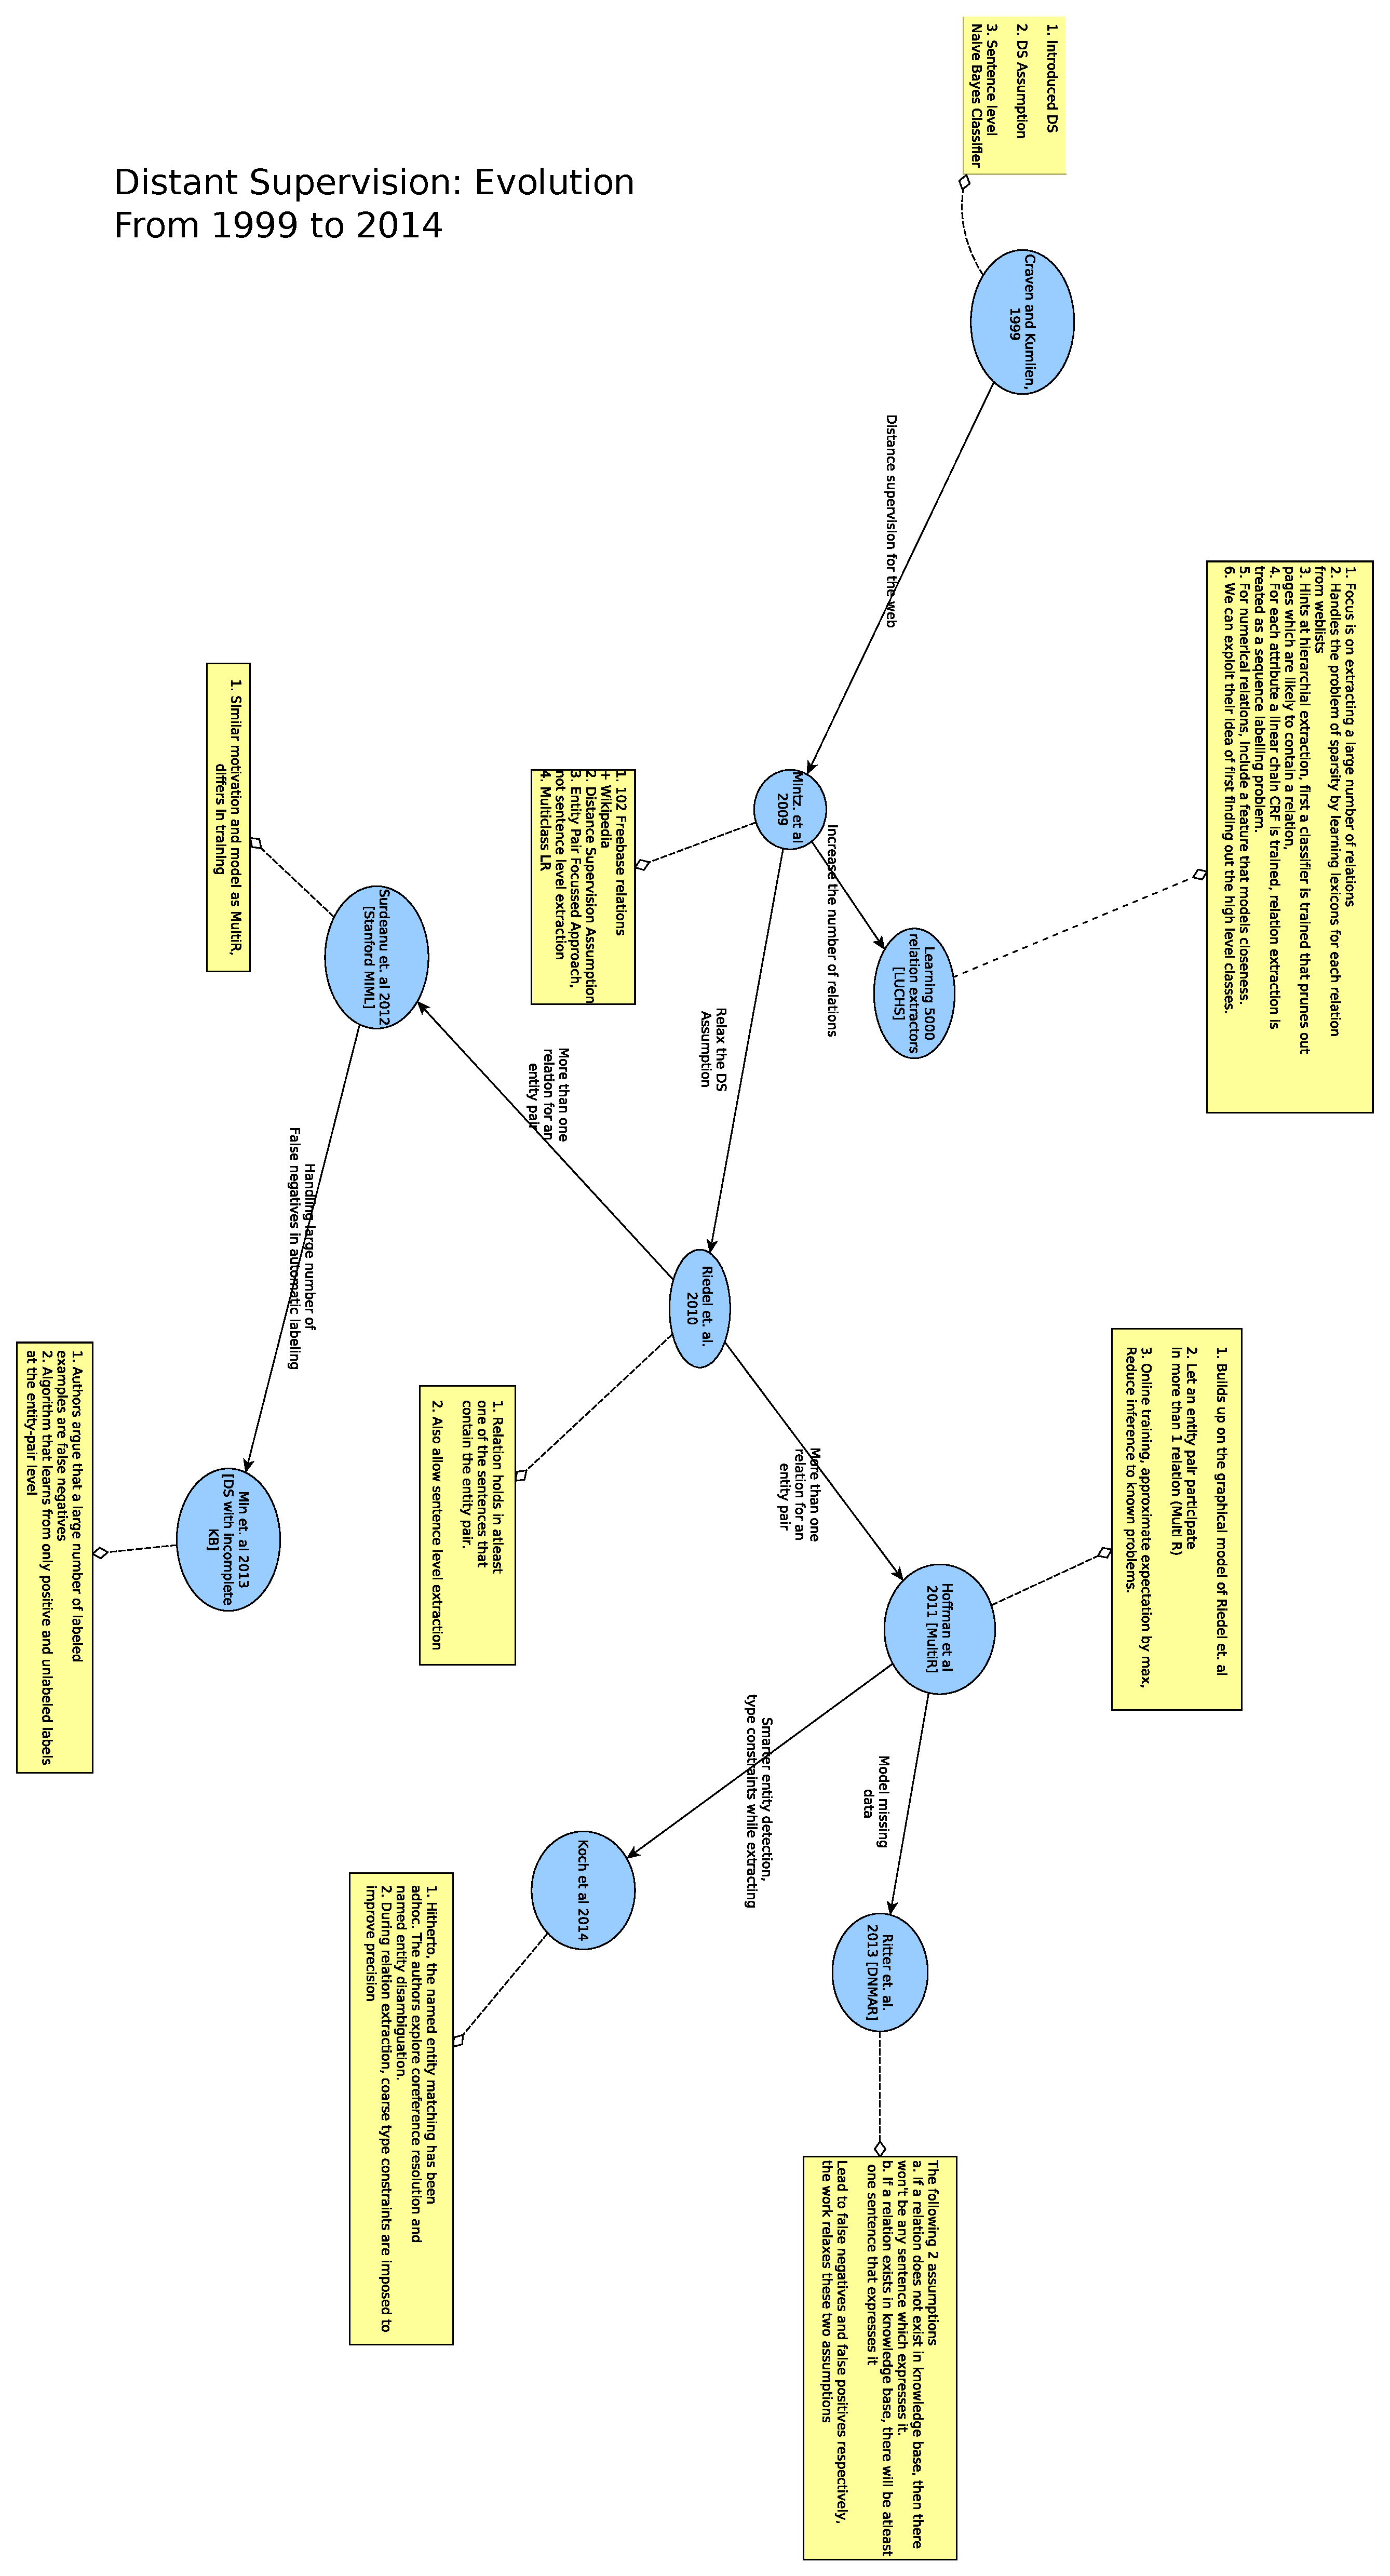
\includepdf[pages={1}]{dsreadings.pdf}
\printbibliography[title=References]
\end{document}
